%
% File acl2020.tex
%
%% Based on the style files for ACL 2020, which were
%% Based on the style files for ACL 2018, NAACL 2018/19, which were
%% Based on the style files for ACL-2015, with some improvements
%%  taken from the NAACL-2016 style
%% Based on the style files for ACL-2014, which were, in turn,
%% based on ACL-2013, ACL-2012, ACL-2011, ACL-2010, ACL-IJCNLP-2009,
%% EACL-2009, IJCNLP-2008...
%% Based on the style files for EACL 2006 by 
%%e.agirre@ehu.es or Sergi.Balari@uab.es
%% and that of ACL 08 by Joakim Nivre and Noah Smith

\documentclass[11pt,a4paper]{article}
\usepackage[hyperref]{acl2020}
\usepackage{times}
\usepackage{latexsym}
\usepackage{multirow}
\usepackage[normalem]{ulem}
\useunder{\uline}{\ul}{}
\renewcommand{\UrlFont}{\ttfamily\small}
\usepackage{booktabs}
\usepackage{graphicx}
\graphicspath{ {../images/} }
\usepackage{subfig}

% This is not strictly necessary, and may be commented out,
% but it will improve the layout of the manuscript,
% and will typically save some space.
\usepackage{microtype}

\aclfinalcopy % Uncomment this line for the final submission
%\def\aclpaperid{***} %  Enter the acl Paper ID here

%\setlength\titlebox{5cm}
% You can expand the titlebox if you need extra space
% to show all the authors. Please do not make the titlebox
% smaller than 5cm (the original size); we will check this
% in the camera-ready version and ask you to change it back.

\newcommand\BibTeX{B\textsc{ib}\TeX}

\title{Twitter Sentiment and Emotion Analysis}

\author{Oihane Cantero \\
  UPV/EHU \\
  \texttt{email@domain} \\\And
  Julen Etxaniz \\
  UPV/EHU \\
  \texttt{email@domain} \\\And
  Jose Javier Saiz \\
  UPV/EHU \\
  \texttt{email@domain} \\}

\date{}

\begin{document}
\maketitle
\begin{abstract}
This corpus is a monolingual resource of unique tweets about product reviews, with each tweet paired with an adversarial sentence. Both original and adversarial tweets are manually and automatically annotated according to sentiment polarity (positive, negative, neutral). The objective is to compare and evaluate both types of annotation.
\end{abstract}

\section{Introduction}

This corpus is a monolingual resource of unique English tweets about technology, with each tweet paired with an adversarial sentence. Both original and adversarial tweets are manually and automatically annotated according to sentiment polarity (positive, negative, neutral) and emotions (joy, anger, sadness, optimism). For automatic annotation, the TweetEval \cite{barbieri-etal-2020-tweeteval} evaluation framework  was used, which covers both sentiment polarity and stance detection for Twitter-specific data, among other classification tasks. The objective is to compare and evaluate both types of annotation.

The aim of this resource is to compare the annotations of tweets about technology and their adversarial sentences. It will also be interesting to compare these annotations when we do it by hand or automatically. The results will show whether the models are affected in their performance on classification tasks when faced with adversarial samples. If performance is significantly compromised by this phenomenon, improvements in the criteria used to generate the models may be proposed.

\section{Related work}

\section{Material and methods}

\subsection{Data statement}

A data statement is a document which serves as the contextualization and description of a data set, usually within the Natural Language Processing context \cite{bender-friedman-2018-data}. It was proposed to make the data sets more understandable for any user and overall, to avoid bad practices within the research and professional practice. In the following sections, we are going to cover the data statement for this corpus so to explain the decisions and reasons behind our work.

The resource and code are publicly available at GitHub\footnote{\url{https://github.com/juletx/twitter-sentiment}}. The code is licensed under the MIT open source license. All non-code materials provided are made available under the terms of the CC BY 4.0 license
(Creative Commons Attribution 4.0 International license).

\subsubsection*{A. CURATION RATIONALE}
The corpus is a monolingual test set intended to evaluate text classification models for their ability to estimate sentiment and emotion. This is based on their performance against regular documents and adversarial phenomena. It contains a sample of 140 tweets about technology obtained from the Twitter API via the Tweepy package. We exclude retweets, quotes and replies to get better tweets. We also exclude tweets that have links to reduce spam tweets. The exact search query used is:  \textit{context:65.848920371311001600 lang:en -is:retweet -is:quote -is:reply -has:links}. The goal for using these parameters to collect the text samples was to obtain as many opinions with pronounced sentiments as possible, so that the manual annotation would be as accurate and homogeneous as possible.

\subsubsection*{B. LANGUAGE VARIETY}
Data extraction was made using the IETF language tag for English \textit{en} (ISO 639-1). This language label does not refer to any geographic region or specific variety of English, but since the demographic group of speakers is mostly from the United States, as explained in the section 3.1-C, the language code is \textit{en-US} (ISO 639-1/ ISO 3166-1 alpha-2), which refers to all American English varieties.

\subsubsection*{C. SPEAKER DEMOGRAPHIC}
Tweets are included upon language and semantic content. Any other type of information or demographic data cannot be controlled for selection, which means that this corpus is not based on specific speakers, but on randomly chosen instances from a larger collection.
Therefore, we must rely on general Twitter demographics, which include a majority of speakers which are male (70.4\%) and ranges between 18 and 49 years old (78.7\%). Tweet metadata sometimes provides location information, which for our sample suggests that a significant number of the instances originate in the United States. This information is relevant for determining the prevailing language variety in the corpus.

\subsubsection*{D. ANNOTATOR DEMOGRAPHIC}
The annotation was made by three Spanish MSc students with training in linguistics and computer science.

\subsubsection*{E. SPEECH SITUATION}
Tweets are characterized by being short, spontaneous and conversational in nature. That is, opinions are concise and sentiments are condensed into a few words, which is important for the corpus because it guarantees that the annotation will be carried out and analyzed accurately. Tweets are also time-sensitive texts, which means that the content the instances is only relevant to the time in which they were written.

\subsubsection*{F. TEXT CHARACTERISTICS}
The sample includes tweets made before February 1. The Twitter context “Interests and Hobbies Vertical: Technology'' (domain and entity ID: 65.848920371311001600) was used as the thematic parameter. This context includes “top-level interests and hobbies groupings” about “technology and computing”, as indicated in the description of the metadata context.

\subsection{Guidelines}

We defined very simple initial guidelines before starting the annotation process. The tweets were annotated according to the sentiment (positive, negative, neutral) and emotion (joy, anger, sadness, optimism) that was inferred by the semantic content. Only one label per tweet is allowed for both tasks. We read tweets one by one and annotate both tags.

After the first annotation, we realized that we needed to update the guidelines to increase the annotator agreement. On the one hand, there were some misunderstandings with words and symbols. For example, \&lt;3 is used as a heart and \&gt; equals greater than. On the other hand, there were some were some cases where specific criteria had to be decided to select a label.

When annotating sentiments, some tweets seemed to be ironic or sarcastic, and it was difficult to decide a tag. Since irony makes the "intended meaning [...] appear on the surface to express the opposite" \cite{OUP2022}, we decided for those cases expressing irony or sarcasm to label the opposite sentiment to the overall sentiment when taken literally. 

Another problem for which a clear guideline was needed was tweets with contradicting sentiments. For this case, we decided to keep the overall sentiment to avoid using too many neutral tags.

When there is no clear emotion, we decided to select the \textit{joy} tag because it is the term with the broadest meaning among the possible options. Also, if there is uncertainty between the \textit{joy} and \textit{optimism} sentiments, we also decided to select \textit{joy} for the same reason.

These guidelines are summarized and exemplified in Table \ref{tab:guidelines}.

\begin{table*}[ht]
\centering
\begin{tabular}{llll}
\hline
\multicolumn{1}{c}{\multirow{2}{*}{\textbf{Problem}}} & \multicolumn{1}{c}{\multirow{2}{*}{\textbf{Guideline}}} & \multicolumn{2}{c}{\textbf{Example}} \\ \cline{3-4} 
\multicolumn{1}{c}{} & \multicolumn{1}{c}{} & \multicolumn{1}{c}{\textbf{Sentence}} & \multicolumn{1}{c}{\textbf{Label}} \\ \hline
Irony/ Sarcasm & \begin{tabular}[c]{@{}l@{}}Use opposite sentiment\\ to the literal one\end{tabular} & \begin{tabular}[c]{@{}l@{}}”oh yeah tesla well what about a\\ car that just logs into your tiktok\\ acct and drives you to starbucks”\end{tabular} & negative \\ \hline
\begin{tabular}[c]{@{}l@{}}Contradicting\\ sentiments\end{tabular} & \begin{tabular}[c]{@{}l@{}}Prefer overall sentiment \\ over the ”neutral” tag\end{tabular} & \begin{tabular}[c]{@{}l@{}}”Finally managed to move my\\ business email from google\\ hosting to another host. So\\ stressful and difficult. The whole\\ internet is so hard! At least the\\ metaverse is coming, I’m confident\\ that will make everything easy and\\ good, phew.”\end{tabular} & positive \\ \hline
Unclear emotion & \begin{tabular}[c]{@{}l@{}}Prefer ”joy” tag for\\ being broader in sense\end{tabular} & \begin{tabular}[c]{@{}l@{}}”All the software I create will be\\ free and open source, but that\\ doesn’t necessarily mean I won’t\\ write cryptic software for some\\ of my projects”\end{tabular} & joy \\ \hline
\end{tabular}
\caption{Defined guidelines after the Inter Annotator Agreement with corresponding examples.}
\label{tab:guidelines}
\end{table*}

\subsection{Inter Annotator Agreement}

Initially, a sample of the first 20 instances was shared among the annotators. The annotations for these initial tweets were used to calculate Inter Annotator Agreement. Table \ref{tab:examples} shows examples of these instances.

\begin{table*}[ht]
\centering
\begin{tabular}{l|lll|lll}
\hline
\multicolumn{1}{c}{\multirow{2}{*}{\textbf{Text}}} & \multicolumn{3}{c}{\textbf{Sentiment}} & \multicolumn{3}{c}{\textbf{Emotion}} \\ \cline{2-7} 
\multicolumn{1}{c}{} & \multicolumn{1}{c}{\textbf{julen}} & \multicolumn{1}{c}{\textbf{oihane}} & \multicolumn{1}{c}{\textbf{javier}} & \multicolumn{1}{c}{\textbf{julen}} & \multicolumn{1}{c}{\textbf{oihane}} & \multicolumn{1}{c}{\textbf{javier}} \\ \hline
\textit{\begin{tabular}[c]{@{}l@{}}just put a CD into my MacBook \\ to burn it and my computer \\ is literally trembling with \\ reawakened recognition\end{tabular}} & negative & positive & negative & anger & joy & joy \\ \hline
\textit{\begin{tabular}[c]{@{}l@{}}oh yeah tesla well what about \\ a car that just logs into your \\ tiktok acct and drives you to \\ starbucks\end{tabular}} & neutral & positive & negative & joy & joy & anger \\ \hline
\textit{\begin{tabular}[c]{@{}l@{}}\#100DaysOfCode Haven’t \\ updated in a while due to not \\ feeling well, just been reviewing \\ some HTML/CSS \&amp; \\ JavaScript until I feel better to \\ take on new concepts. Also \\ been watching mock interviews :)\end{tabular}} & negative & negative & negative & sadness & optimism & optimism \\ \hline
\end{tabular}
\caption{Instance examples used to calculate Inter Annotator Agreement.}
\label{tab:examples}
\end{table*}

Table \ref{tab:agreement} shows that there is moderate agreement and a low Kappa score in the first results. The agreement results in the sentiment task are homogeneous between pairs, while in the emotion task the results were more varied. This is explained by the task labels: the sentiment task uses labels which are more clear, while the labels in the emotion task are more subjective and open to interpretation. This is main reason why the guidelines were updated, after which the annotation was repeated along the Inter Annotator Agreement calculation. The results for the annotations with the updated guidelines show a clear improvement in the emotion task.

\begin{table*}[ht]
\begin{tabular}{lrrrr}
\toprule
        pairs &  agreement\_sentiment &  kappa\_sentiment &  agreement\_emotion &  kappa\_emotion \\
\midrule
 julen oihane & 70.0 $\rightarrow$ \textbf{65.0} & 53.8 $\rightarrow$ \textbf{45.1} & 55.0 $\rightarrow$ \textbf{70.0} & 33.3 $\rightarrow$ \textbf{49.2} \\
 julen javier & 60.0 $\rightarrow$ \textbf{70.0} & 40.1 $\rightarrow$ \textbf{49.4} & 40.0 $\rightarrow$ \textbf{70.0} & 13.0 $\rightarrow$ \textbf{46.9} \\
javier oihane & 60.0 $\rightarrow$ \textbf{55.0} & 39.2 $\rightarrow$ \textbf{32.3} & 65.0 $\rightarrow$ \textbf{70.0} & 46.2 $\rightarrow$ \textbf{50.0} \\
\midrule
      average & 63.3 $\rightarrow$ \textbf{63.3} & 44.4 $\rightarrow$ \textbf{42.3} & 53.3 $\rightarrow$ \textbf{70.0} & 30.8 $\rightarrow$ \textbf{48.7} \\
\bottomrule
\end{tabular}
\caption{Inter Annotator Agreement result improvements after updating the guidelines. Final results are in bold.}
\label{tab:agreement}
\end{table*}

Thereafter each annotator was given a different set of 40 tweets for annotation. The same methodology was followed, where the manual annotations were used to evaluate the accuracy of the models.

\subsection{Automatic annotation}

These tweets were also labelled using automatic models. Models trained for the TweetEval \cite{barbieri-etal-2020-tweeteval} evaluation framework were used. This framework covers many classification tasks that include sentiment and emotion classification. 

The base RoBERTa \cite{liu2019roberta} model was pretrained using 58M English tweets. Then each model is finetuned using specific data for that task. SemEval 2017 Subtask A data \cite{rosenthal2019semeval} is used for sentiments and SemEval 2018 Affects in Tweets \cite{mohammad-etal-2018-semeval} is used for emotions.

The fine-tuned models are available in HuggingFace and that makes them very easy to use. They only require a small preprocessing step to substitute all mentions with @user and links with http.

\subsection{Adversarial examples}

We will create some adversarial tweets automatically to measure the impact in the metrics of the models. The aim of these adversarial examples is to confuse the models while maintaining the manual label. Therefore, if we generate the adversarial examples correctly, they should have the same meaning and sense, so there is no need to annotate them. As these attacks can easily be replicated, we decided not to include them in the final resource.

We used the Adversary\footnote{\url{https://github.com/airbnb/artificial-adversary}} library to generate 8 generic attacks. These attacks are not specifically prepared for our models, they are simple attacks that can be tested on any type of model. Words are selected with a probability of 0.3 and the selected attack is applied to those words. Attacks can also be combined, but we decide to apply them separately for simplicity. An example of each attack can be seen in Table \ref{tab:adversarial}. This tweet was manually annotated as negative sentiment and anger emotion.

\begin{table*}[ht]
\centering
\begin{tabular}{llll}
\hline
\multicolumn{1}{c}{\multirow{2}{*}{\textbf{Type}}} & \multicolumn{1}{c}{\multirow{2}{*}{\textbf{Sentence}}} & \multicolumn{2}{c}{\textbf{Label}} \\ \cline{3-4} 
\multicolumn{1}{c}{} & \multicolumn{1}{c}{} & \multicolumn{1}{c}{\textbf{Emotion}} & \multicolumn{1}{c}{\textbf{Sentiment}} \\ \hline
Original & having no sort of WiFi actually sucks & negative & sadness \\
Swap words & having no sort WiFi of actually sucks & negative & sadness \\
Remove space & having-no`sort of WiFi actually sucks & negative & anger \\
Replace letters with symbols & having no \$or7 of WiFi actually \$u\{[\}kS & neutral & sadness \\
Swap letters & having no srot of WiFi actually sucks & negative & anger \\
Insert punctuation & having no sor{]}\{t of WiFi actually {]}su!cks & neutral & sadness \\
Insert duplicate characters & having no sorttt of WiFi actually sucks & negative & sadness \\
Delete characters & having no sot of WiFi actually sucks & negative & sadness \\
Change case & having no SORT of WiFI actually sucks & negative & anger \\ \hline
\end{tabular}
\caption{Examples of adversarial sentences and the predicted sentiment and emotion.}
\label{tab:adversarial}
\end{table*}

\section{Results}

We will compare the results and extract some conclusions about the performance of the models. We will visualize the percentage of tweets from each class in the manual and automatic annotations. We will also visualize the most common words of each class in word clouds.

\subsection{F1 scores}

F-score was calculated for each label and macro-average for all labels in each task in order to compare the model results against the manual annotations. 
As can be seen in Table \ref{tab:f1_scores}, the results with adversarial sentences output lower F-scores than with the original sentences. For the sentiment task, the performance with original sentences delivers a 65.8 F-score against a 61.7 mean F-score with the adversarial sentences. The same applies to the emotion task results, which bring a 53.3 F-score with original sentences and a 50.7 mean F-score with the adversarial sentences.
Even if in overall results for adversarial sentences are worse than the original ones, we can remark that some of the adversarial attacks doesn't decrease F-score, they even improve it in some cases. The best results for sentiment analysis are for the \textit{swap\_words} attack and this same attack performs quite well in emotion detection. And for emotion detection the best results are for \textit{remove\_spacing}, that doesn't receive so bad results for sentiment analysis. So watching these results, we may conclude that removing a space of the sentence or word order doesn't really matter for these tasks.

In Figure \ref{fig:barplots}, we see the results of Table \ref{tab:f1_scores} into barplots, we see the score differences between each tag. The tag that is classified worse for both original and adversarial sentences is \textit{positive}, and for emotions, we see that \textit{anger} and \textit{joy} are the tags that get better results, and \textit{optimism} is clearly below all the others.

In Figure \ref{fig:barplot}, we can observe that between the two tasks, sentiment analysis get better results for both original and adversarial sentences.

And in Figure \ref{fig:scatterplot}, we can see the difference in scores between the two tasks and all the adversarial attacks. 

%See Figures \ref{fig:barplots}, \ref{fig:barplot} and \ref{fig:scatterplot}.

%mark best results in bold

\begin{table*}[ht]
\centering
\begin{tabular}{l|rrr|r|rrrr|r}
\toprule
                       text &  neg &  neu &  pos &  sen &  ang &  joy &  opt &  sad &  emo \\
\midrule
                       original &      71.0 &     71.0 &      70.3 &       65.8 &   66.7 & 66.1 &      27.9 &     52.6 &     53.3 \\
                 swap\_words &      \textbf{73.1} &     \textbf{73.1} &      \textbf{71.0} &       \textbf{67.2} &   67.6 & 64.6 &      27.9 &     51.3 &     52.8 \\
             remove\_spacing &      68.2 &     68.2 &      60.2 &       61.2 &   \textbf{69.6} & \textbf{68.2} &      33.3 &     \textbf{55.0} &     \textbf{56.5} \\
           letter\_to\_symbol &      65.2 &     65.2 &      58.5 &       59.0 &   62.5 & 62.0 &      22.9 &     38.9 &     46.6 \\
               swap\_letters &      69.0 &     69.0 &      64.3 &       62.8 &   67.6 & 64.1 &      21.6 &     31.6 &     46.2 \\
         insert\_punctuation &      62.8 &     62.8 &      55.7 &       57.5 &   62.5 & 74.0 &      20.0 &     35.0 &     47.9 \\
insert\_duplicate\_characters &      72.5 &     72.5 &      63.6 &       63.9 &   66.7 & 66.7 &      26.3 &     47.4 &     51.8 \\
          delete\_characters &      68.2 &     68.2 &      59.5 &       59.9 &   68.5 & 66.7 &      27.8 &     41.0 &     51.0 \\
                change\_case &      71.1 &     71.1 &      63.6 &       62.6 &   63.2 & 65.6 &      \textbf{37.2} &     44.4 &     52.6 \\
\bottomrule
\end{tabular}
\caption{F1 scores for original text and adversarial attacks. F1 for each label and macro-average of all labels for sentiment and emotion.}
\label{tab:f1_scores}
\end{table*}

\begin{figure*}[ht]
    \centering
    \subfloat{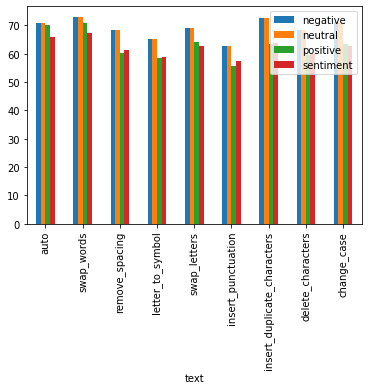
\includegraphics[width=0.49\linewidth]{barplot_sentiment.png}}
    \subfloat{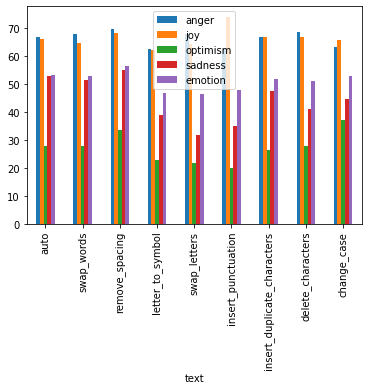
\includegraphics[width=0.49\linewidth]{barplot_emotion.png}}
    \caption{F1 for each label and macro-average of all labels for sentiment and emotion.}
    \label{fig:barplots}
\end{figure*}

\begin{figure}[ht]
    \centering
    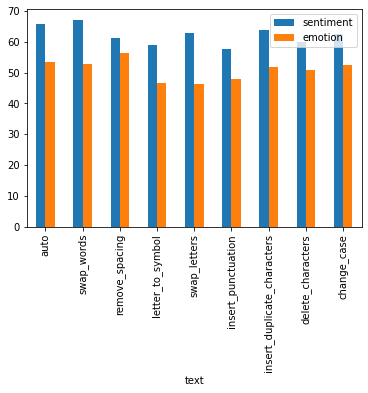
\includegraphics[width=\linewidth]{barplot_sentiment_emotion.png}
    \caption{Sentiment and emotion barplot.}
    \label{fig:barplot}
\end{figure}

\begin{figure}[ht]
    \centering
    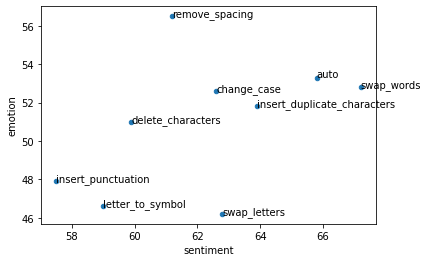
\includegraphics[width=\linewidth]{scatterplot_sentiment_emotion.png}
    \caption{Sentiment and emotion scatterplot.}
    \label{fig:scatterplot}
\end{figure}

\subsection{Pieplots}

In Figure \ref{fig:pieplots_sentiment} we can see the distribution of each of the tags of the sentiment analysis task. In the manual distribution, positive and negative tags are equally distributed, and are less neutral tags. In the automatic annotation, the distribution of positive and negative tags are also equally distributed, but the majority class is neutral. This can be because while manually annotating, we tend to avoid neutrality, and we try to put a positive or negative tag at all costs. Another reason may be that we decided to take the overall sentiment when there are positive and negative sentiments in the same tweets, and maybe the model makes an average and classifies them as neutral.

In Figure \ref{fig:pieplots_emotion}, we can see that something similar appends. In our guidelines, we decided that we will put the joy tag when we will have doubts. This increased our manual annotations' joy tags number. For optimism and anger, the results are quite similar but for anger, because the automatic annotation puts more than the manual one. This should be because our guidelines implies that there will be more joy, because we put it when there is no emotion and when we had doubts between joy and optimism, as we think that it is the more general emotion. 

%See Figures \ref{fig:pieplots_sentiment} and \ref{fig:pieplots_emotion}.

\begin{figure*}[ht]
    \centering
    \subfloat{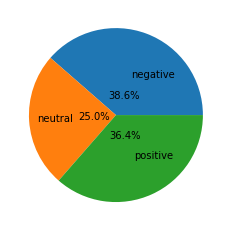
\includegraphics[width=0.49\linewidth]{pieplot_sentiment_manual.png}}
    \subfloat{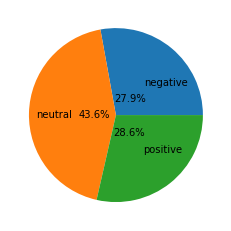
\includegraphics[width=0.49\linewidth]{pieplot_sentiment_auto.png}}
    \caption{Sentiment label percentages for manual and automatic annotation.}
    \label{fig:pieplots_sentiment}
\end{figure*}

\begin{figure*}[ht]
    \centering
    \subfloat{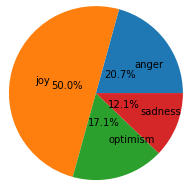
\includegraphics[width=0.49\linewidth]{pieplot_emotion_manual.png}}
    \subfloat{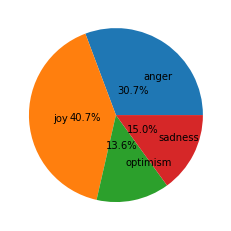
\includegraphics[width=0.49\linewidth]{pieplot_emotion_auto.png}}
    \caption{Sentiment label percentages for manual and automatic annotation.}
    \label{fig:pieplots_emotion}
\end{figure*}

\subsection{Wordclouds}

\section{Conclusions}

Classification tasks in Twitter related to sentiment analysis have grown in importance over the last years, and with an increasing number of models and frameworks created around this tasks, it is worth evaluating the implementation of these methods. 

Our evaluation focuses on the outcomes of a popular Twitter-specific framework across two tasks by comparing its results to human annotation. This evaluation method is useful for the purpose of this work because it allows us to examine the broader potential impact of these models and whether the guidelines used to create the training corpus for these tasks translate into adequate performance on sentiment analysis tasks.

We saw that good guidelines are essential to annotate manually, even if the task seems to be "easy". They allow annotators to annotate the same way, and are very important if we want to create a coherent resource. 

The outcomes of this work have shown that classification models have multiple sources of error and tend to under-perform when facing different scenarios such as unknown words, lexicon gaps or unspecified sentence contexts. This shows there is room for improvement in this task. For future work, it would be useful to analyze the performance of the models in multiple other related tasks, such as irony/ sarcasm detection or hate detection, instead of a pair of tasks. Other improvements on this evaluation would be to explore additional languages and other classification frameworks with different guidelines.

\bibliography{twitter_sentiment_emotion}
\bibliographystyle{acl_natbib}

\end{document}
